\documentclass[12pt]{article}

\usepackage{geometry}
\usepackage[utf8]{inputenc}
\usepackage[T2A]{fontenc}
\usepackage[russian]{babel}
\usepackage{graphicx}
\usepackage{caption}
\usepackage{amssymb, gensymb, amsmath}
\usepackage{mathrsfs}
\usepackage{array, colortbl}
\usepackage{multicol}

\title{{\bf Лабораторная работа 8.\, 1. \\ Определение постоянных Стефана-Больцмана и Планка из анализа теплового излучения накаленного газа}}
\author{Лось Денис (группа 618)}
\date{12 октября 2018}

\begin{document}

\maketitle

\paragraph{Цель работы: } при помощи модели абсолютно чёрного тела (АЧТ) провести измерения температуры оптическим пирометром с исчезающей нитью и термопарой, исследовать излчения накаленных тел с различной испускательной способностью, определить постоянные Планка и Стефана-Больцмана.

\section*{Теоритическое введение}
\par
	Закон Стефана-Больцмана для абсолютно чёрного тела
\[
	W = \sigma S \left(T^4 - T_0^4 \right)
\]
\par
	Для серого тела
\[
	W = \varepsilon_T \sigma T^4
\]
\par
	Постоянная Стефана-Больцмана
\[
	\sigma = \frac{2 \pi^5 k_\text{Б}:4}{15 с^2 h^3} = 5.67 \cdot 10^{-12} \, \frac{\text{Вт}}{\text{см}^2 K^4}
\]
\par
	Постоянная Планка выражается как
\[
	h = \sqrt[3]{\frac{2 \pi^5 k_\text{Б}^4}{15 c^2 \sigma}}
\]

\section*{Изучение работы оптического пирометра}
\par
	В данной части работы с помощью пирометра измеряется температура модели АЧТ и проводится сравнение её значения со значением температуры, измеренного при помощи термопарного термометра.
\par
	Учитывая, что постоянная термопары $k = 41 \, \frac{\text{мкВ}}{\text{\degree C}}$, а комнатная температура $T_\text{комн} \approx 20 \degree C$, проведём измерения
\begin{table}[h!]
	\centering
	\begin{tabular}{|c|c|c|}
	\hline
		$T$, \degree C & $U$, мВ & $T_\text{терм}$, \degree C \\
	\hline
		1128 & 43.94 & 1092 \\
	\hline
		1103 & 44.47 & 1105 \\
	\hline
		1108 & 44.51 & 1106 \\
	\hline
		1101 & 44.59 & 1108 \\
	\hline
		1116 & 44.60 & 1108 \\
	\hline
		1110 & 44.60 & 1108 \\
	\hline
	\end{tabular}
	\caption{Измерения для модели абсолютно чёрного тела}
\end{table}
\par
	В результате получим результат, усреднив по лучшим измерениям
\begin{align*}
	T &= \left(1106 \pm 2 \right) \, \text{\degree C} \\
	T_\text{терм} &= \left(1106 \pm 1\right) \, \text{\degree C} \\ 
\end{align*}
\par
	Найденная с помощью пирометра температура c запасом лежит в пределах погрешности $1$ \% от найденной с помощью термопары. 

\section*{Измерение яркостной температуры накаленных тел}
\par
	Этот эксперимент предполагает показать, что различные тела, накаленные до одинаковой термодинамической температуры, имеют различную яркостную температуру.
\par
	Проведём измерения для определения яркостной температуры образцов: трубки и кольца.
\begin{table}[h!]
	\centering
	\begin{tabular}{|c|c|}
	\hline
		$T_\text{трубки}$, \degree C & $T_\text{кольца}$, \degree C \\
	\hline
		863 & 776 \\
	\hline
		856 & 773 \\
	\hline
		858 & 776 \\
	\hline
	\end{tabular}
	\caption{Измерения для определения яркостной температуры образцов}
\end{table}
\par
	Усреднив полученные результаты, получим, что
\begin{align*}
	T_\text{трубки} &= \left(859 \pm 2\right) \text{\degree C} \\
	T_\text{кольца} &= \left(775 \pm 1\right) \text{\degree C} \\
\end{align*}

\section*{Проверка закона Стефана-Больцмана}
\par
	Приведём таблицу с усреднёнными основными измерениями, при этом определяя $\varepsilon_T$ из приведённой в описании таблицы для вольфрама
\begin{table}[h!]
	\centering
	\begin{tabular}{|c|c|c|c|c|c|c|c|c|c|}
	\hline
		$T$, \degree C & 997& 1101& 1202& 1305& 1411& 1501& 1607& 1698& 1802 \\
	\hline
		$I$, А & 0.25 & 0.30 & 0.33 & 0.41 & 0.52 & 0.65 & 0.82& 0.91 & 1.15 \\
	\hline
		$U$, В & 3.35 & 3.74 & 3.95 & 4.06 & 4.92 & 5.08 & 5.50 & 6.60 & 7.82 \\
	\hline
		$W$, Вт & 0.82 & 1.08 & 1.27 & 1.62 & 2.50 & 3.30 & 4.46 & 6.02 & 8.98 \\
	\hline
		$T_\text{терм}$, \degree C & 1020 & 1130 &  1240 & 1350 & 1455 & 1560 & 1670 & 1775 & 1880 \\
	\hline
		$\varepsilon_T$ & 0.105 & 0.119 & 0.133& 0.144 & 0.164 & 0.179 & 0.195 & 0.209 & 0.223 \\
	\hline
	\end{tabular}
\end{table}
\par
	Представим зависимость $W = f(T_\text{терм})$ на графике
\begin{figure}[h!]
	\centering
	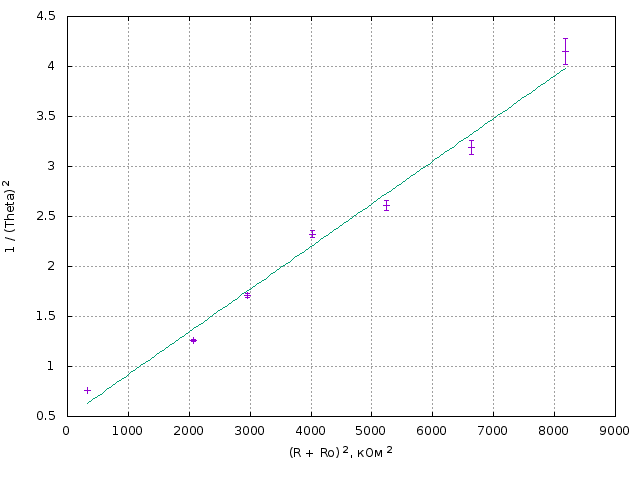
\includegraphics[width = 12cm, height = 7cm]{plot1.png}
	\caption{График зависимости $W = f(T)$}
\end{figure}
\par
	Для для того чтобы убедиться в правильности закона Стефана-Больцмана построим зависимость в логарифмическом масштабе $\ln W = \ln \left(e_T B\right) + n \ln T$. Определим величину $n$ как тангенс угла наклона прямой в области высоких температур,когда мощность подводимая к нити, практически полностью расходуется на излучение.
\par
	Ясно, что $B = S \cdot \sigma$, где $S$ --- эффективная площадь излучающей поверхности нити лампы при температуре более $1500$ \degree C, когда вся нить одинакова накалена; $\sigma$ --- постоянная Стефана-Больмана; $S = 0.36$ $\text{см}^2$.
\begin{figure}[h!]
	\centering
	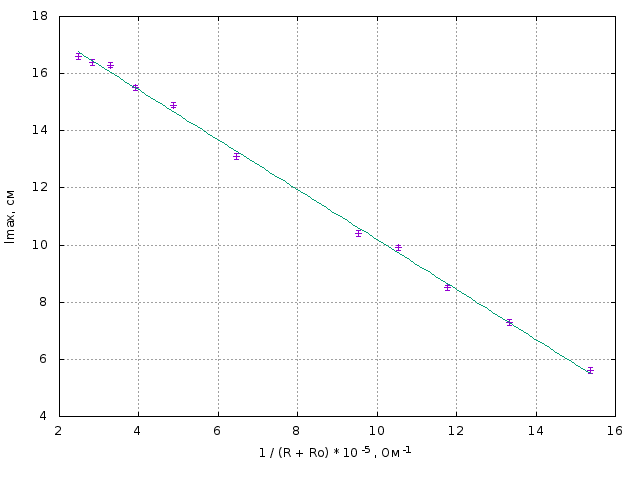
\includegraphics[width = 12cm, height = 7cm]{plot2.png}
	\caption{График зависимости $\ln(W) = f(\ln(T))$}	
\end{figure}
\par
	Проведя прямую по методу наименьших квадратов, определим значение $n$.
\[
	n = \left(3.9 \pm 0.3 \right)
\]
\par
	Так как $n \approx 4$, то следовательно, мы можем говорить о выполнении закона Стефана-Больцмана. Определим величину постоянной Стефана-Больцмана по формуле
\[
	\sigma = \frac{W}{\varepsilon_T S T^4}
\]
для каждого измеренного значения $T_\text{терм}$, превышающего $1700$ \degree C.
\begin{table}[h!]
	\centering
	\begin{tabular}{|c|c|c|c|c|}
	\hline
		$T_\text{терм}$ & $W$, Вт & $\varepsilon_T$ & $\sigma \cdot 10^{-8}$, $\text{Вт} \cdot \text{м}^{-2} \cdot \text{К}^{-4}$ & $\Delta \sigma \cdot 10^{-8}$, $\text{Вт} \cdot \text{м}^{-2} \cdot \text{К}^{-4}$ \\
	\hline
		1698 & 6.02 & 0.209 & 8.1 & 0.3 \\
	\hline
		1802 & 8.98 & 0.223 & 8.9 & 0.4 \\
	\hline
	\end{tabular}
\end{table}
\par
	Полученные значения по порядку величины совпадают с табличным значением постоянной Стефана-Больцмана, однако точное численное значение имеет достаточно серьёзное расхождение.
\par
	Из найденных значений постоянных Стефана-Больмана найдём значение постоянной Планка
\[
	h = \left(5.8 \pm 0.2 \right) \cdot 10^{-34} \cdot \text{Дж} \cdot \text{с}
\]
\par
	Порядок найденной постоянной Планка совпадает с порядком табличного значения, однако как и для постоянных Стефана-Больцмана, мы получили довольно существенное количественное расхождение.

\section*{Измерение яркостной температуры неоновой лампочки}
\par
	Проведём серию измерения для определения яркостной температуры неоновой лампочки
\begin{table}[h!]
	\centering
	\begin{tabular}{|c|c|c|c|c|c|}
	\hline
		$T$, \degree C & 853 & 846 & 841 & 840 & 845 \\
	\hline
	\end{tabular}
\end{table}
\par
	Следовательно, полученное значение яркостной температуры неоновой лампочки
\[
	T_\text{ярк} = \left(845 \pm 3 \right) \, \text{\degree C}
\]
\par
	Однако, если дотронутся рукой до неоновой лампочки, то можно обнаружить, что её термодинамическая температура не совпадает с яркостной. Неоновая лампа относится к числу газоразрядных истчников света. Атомы, входящие в состав инертного газа, наполняющего лампу, переходят в возбуждённое состояние при подачи напряжения, однако они не могут находиться в этом состоянии долгое время. Поэтому через достаточно короткий промежуток времени порядка миллионных долей секунды атом из возбждённого состояния переходит обратно в основное состояние. При обратном переходе происходит излучение энергии в виде кванта света-фотона.

\end{document}